\chapter{OVERLAPPED SPEECH IN SPEAKER RECOGNITION}
\label{chapter:ovl_in_sid}
Detecting overlapped segments has previously been considered in speaker recognition diarization~\cite{boakye_thesis,yantorno_report}. 
In such problems, the presence of a secondary speaker either decreases model reliability (in training), or introduces confusion in the decision-making process by distorting test files. 
Overlap detection is computationally advantageous when compared to enhancing the desired speaker's speech. 
This approach is especially useful when one has the luxury of neglecting overlapped data~\cite{yantorno_report}. 
Such is the case for speaker recognition and diarization~\cite{Boakye_is_08}. 
By detecting overlapped speech segments, we are able to remove them from the training and decision-making process. However, overlap removal will not be the approach of choice in this chapter. 

As pointed out in Chapter~\ref{chapter:front-end}, the downside in removing overlapped segments is that a considerable amount of ``usable'' speech is also omitted from the speaker recognition system. 
An alternative solution is investigated in this chapter. 
In this solution, instead of directly applying overlap detection to data, overlap detection decisions are used as quality measure scores to assist speaker verification performance. 
This method is investigated in Sect.~\ref{sec:ch2_OvlQualityMeasure}. 
The primary contribution of this study is therefore to:
\begin{itemize}
	\item investigate overlap detection scores as quality measures for speaker verification. 
\end{itemize}
But first, this chapter begins by demonstrating the effects of overlapped data on speaker verification experiments (Sect.~\ref{sec:ch3_SIDintro}). 
This will provide an understanding of how overlaps affect speaker recognition. 
In addition, we will see how introducing overlaps to speaker verification affects train and test data separately (Sect.~\ref{sec:ch3_OvlinTest}~and~\ref{sec:ch3_OvlinTrain}). 


\section{Investigative setup}
\label{sec:ch3_SIDintro}
In order to show the detrimental effects of adding overlapped data to speaker verification, a case study is presented to analyze speaker recognition on data from the monaural speech separation challenge described in Chapter~\ref{chapter:front-end}~\cite{cooke20101}. 
Experiments use $12$-dimensional MFCC features ($13$ excluding the $0^{th}$ coefficient) plus $\Delta$ and $\Delta\Delta$, which together result in $36$-dimensional features. 
The experiments use the Gaussian mixture model (GMM) approach where a trained speaker is modeled using a mixture of Gaussians and the maximum likelihood of a given test audio file is computed from the train model. 
GMM parameters are obtained through maximum a-posterior adaptation of the parameters of a speaker independent GMM (called a universal background model which is trained on a large pool of speakers). 
Only GMM means are MAP-adapted in these experiments. 
$512$ mixtures were used to form the Universal background model (UBM). 

The next section slightly digresses from overlapped speech and is intended for readers unfamiliar with speaker recognition frameworks. 
Readers that feel comfortable with the concepts of speaker verification, specifically the use of GMM-UBM setups for speaker for verification, may skip Sect.~\ref{ssec:ch3_GMMUBM}.

As mentioned above, trials are generated from train and test sets designed for the speech separation challenge. 
The amount of clean (i.e., single-speaker) training data for each speaker is approximately $15$ minutes. 
Test data are provided in six SIR conditions, which are evaluated separately (see Sect.~\ref{sec:ch3_OvlinTest}). 
The challenge also provides overlapped training data. 
Overlapped training data are used in Sect.~\ref{sec:ch2_OvlinTrain} to train speaker models with the main speaker (i.e., model speaker in each train file) as the primary speaker and interfering speech from another randomly selected speaker. 
Experiments are gender-dependent, therefore the number of female speakers and male speakers is slightly different. 
In total over $10000$ trials are used to calculate equal error rates for each SIR condition presented in Sect.~\ref{sec:ch3_OvlinTest} and Sect.~\ref{sec:ch3_OvlinTrain} with a target to non-target ratio of $0.001$. 

\subsection{Speaker verification in a GMM-UBM setup} 
\label{ssec:ch3_GMMUBM}
The speaker verification problem is a manifestation of the more generic problem of speaker recognition in the form of a binary detection problem. 
Speaker recognition, taken literally, implies sufficient knowledge of all speakers (or at least a large number of speakers) to ``recognize'' a given speaker from his/her voice. 
Speaker verification, on the other hand, tackles the more manageable problem of determining whether an audio segment was produced by a known speaker. 
A speaker verification system usually produces a likelihood value for each verification task (aka trial). 
The collection of trial likelihood values produces two distributions, one of which corresponds to true (aka target) trials and the other to imposter (aka non-target) trials. 

The described framework requires a model for the training speakers (for whom we have several recording sessions available), but for the test speakers we only use the features from a test audio signal to compute the maximum likelihood (ML) probability of the test speaker belonging to the corresponding train speaker in each trial. 
Figure~\ref{fig:speaker_verification} summarizes a speaker verification setup. 

\begin{figure}[h!]
	\centering
	\vspace{0mm}
	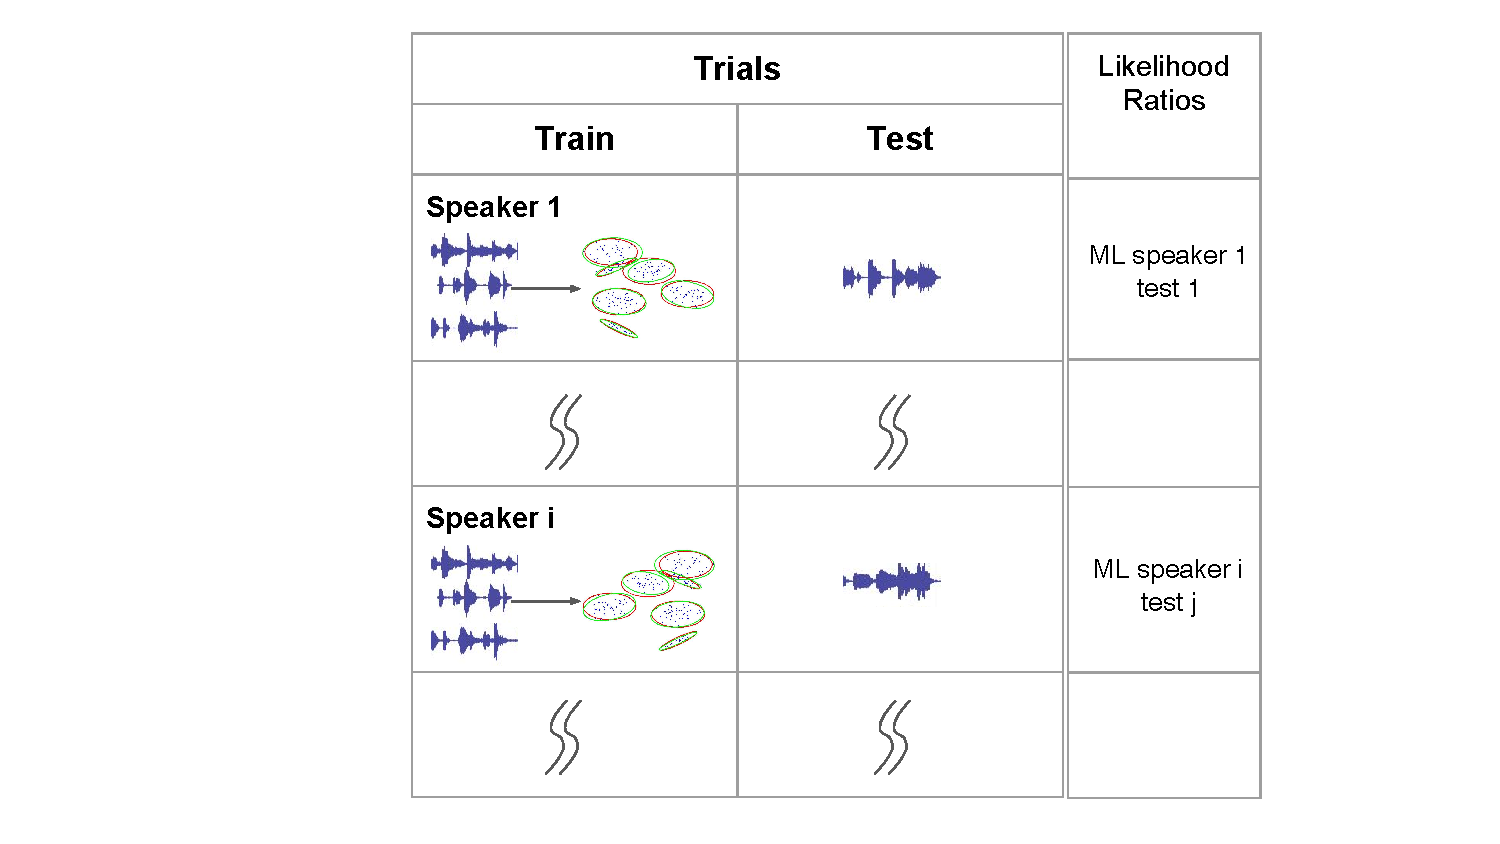
\includegraphics[height = 3in, width=0.8\textwidth]{figures/speaker_verification_setup}
	\vspace{-3mm}
	\caption{\it Speaker verification setup}
	\label{fig:speaker_verification}
	\vspace{0mm}
\end{figure}

The method through which likelihood ratios are calculated varies depending on the choice of model and system specifics. 
In the experiments presented in the following section, we use a GMM-UBM system~\cite{reynolds_map}. 
As mentioned above the task of the verification system is to calculate the likelihood of a test audio belonging to a speaker model. 
In other words, if the test audio belongs to speaker $i^\prime$ and the model (i.e., training speaker) belongs to speaker $i$, the objective is to calculate the likelihood of $i=i^\prime$. 
Here, a model is a Gaussian mixture model (GMM) obtained by adapting means of a universal GMM (aka UBM). 
The UBM is trained on background development data. 
In the examples provided in Sect.~\ref{sec:ch3_OvlinTest}~and~\ref{sec:ch3_OvlinTrain}, the development data is TIMIT. 
The verification system considers to hypotheses: 1) the probability of the test audio being generated from $GMM_i$, 2) the probability of the test audio generated from the UBM, which in this case represents every other speaker except $i$. 
The ratio between these two ratios is used to quantify the system decision for a given trial. 
Figure~\ref{fig:gmm_ubm_sid} illustrates the procedure to determine the likelihood ratio for one trial. 

\begin{figure}[h!]
	\centering
	\vspace{0mm}
	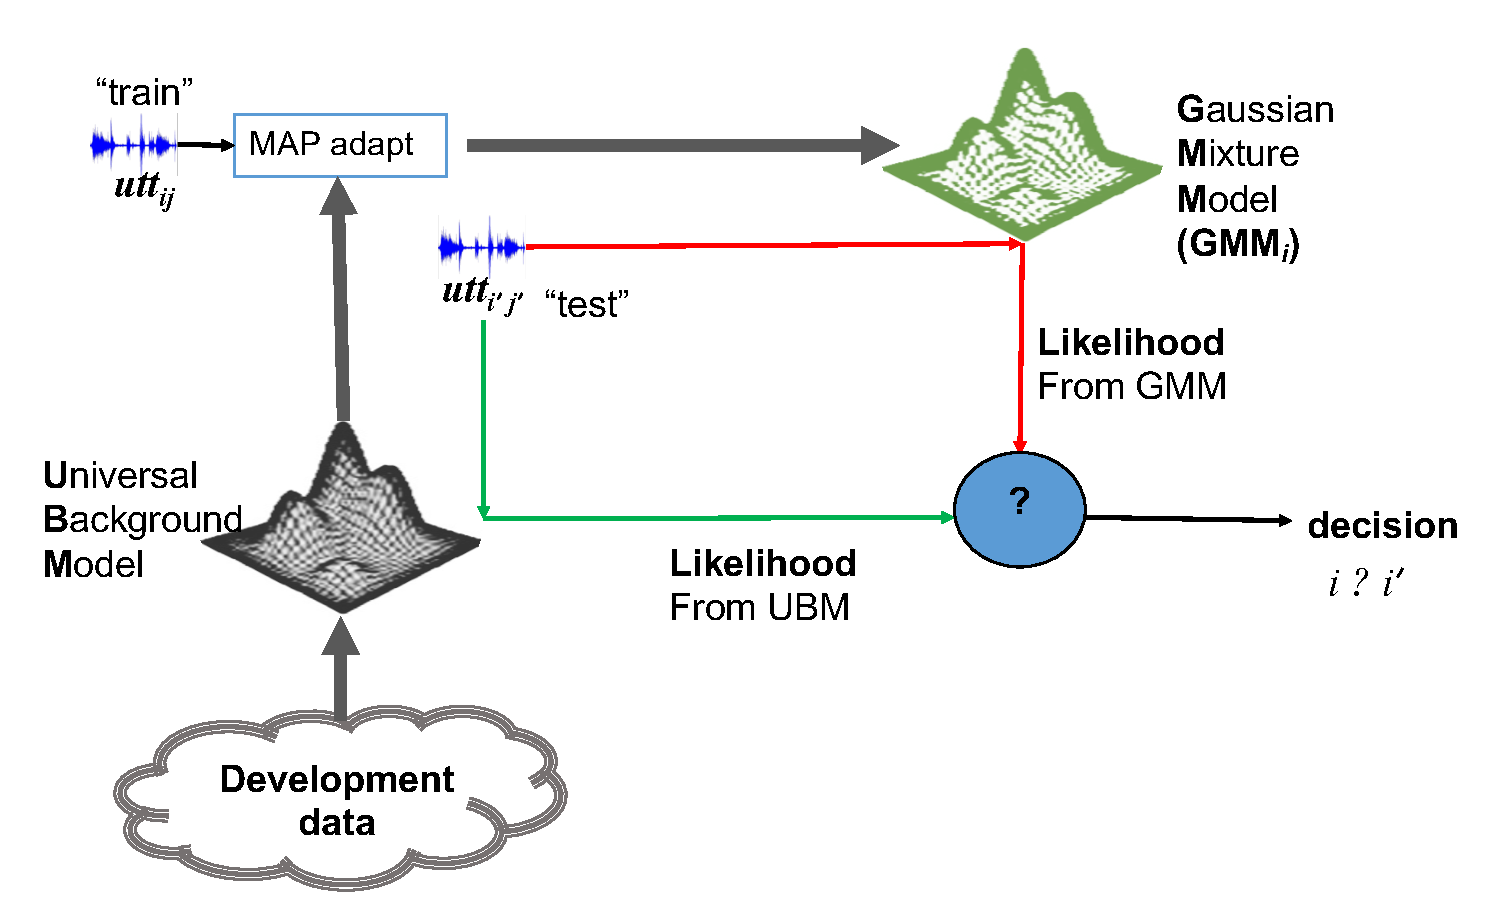
\includegraphics[height = 3.5in, width=0.9\textwidth]{figures/gmm_ubm_sid_setup}
	\vspace{-3mm}
	\caption{\it Speaker verification setup}
	\label{fig:gmm_ubm_sid}
	\vspace{0mm}
\end{figure}

Given this introduction, we expect that the reader should now be able to follow the remainder of this chapter. 
Useful descriptions of topics on speaker verification and recognition can be found in~\cite{hansen2015SIDmagazine}. 


\section{Overlaps in test data}
\label{sec:ch3_OvlinTest}
As a comparison benchmark, performance is evaluated under clean train and test conditions on the SSC data. 
Gaussian mixture models (GMM) are adapted from a Universal back model (UBM) trained on TIMIT files~\cite{msridentity}. 
For each model (training) speaker, there are 500 utterances in SSC, which are all used in the training process. Test files are available in all SIR conditions. 
As expected, lower SIR values correspond to higher equal error rates. 
The presence of a secondary speaker, clearly causes confusion in the score distribution, leading to less separability between target and imposter trials. 
recognition performance under clean test files and those with average SIR ranging in $+6, +3, 0, -3, -6, -9 dB$ are provided in Fig.~\ref{fig:sidingrid_ovlintest_train_a}. 

It is worth mentioning that it was tempting to compare these results with stationary noise experiments. 
However, contrary to expectations, it was observed that performances were better in the overlapped condition when compared to white Gaussian noise and speech-shaped noise interference, even for negative SIR values. 
This is most likely due to a misunderstanding caused by comparing stationary and non-stationary noise through the same measurement procedure, which is the SIR (or SNR). 
For a given target speech file, adding a certain amount of stationary noise will affect all frames, whereas in the case of non-stationary noise (here speech) only a portion of the frames receive non-uniform interference. 
This leads to incomparable results under presumably similar conditions which we decided to exclude from this study to avoid confusion. 
Therefore, an important take-away message here is that a certain {\bf SIR} value does not translate to the same {\bf SNR}. 


\section{Overlap in train data}
\label{sec:ch3_OvlinTrain}
This section examines the effect of adding overlapped speech to train files (Fig.~\ref{fig:sidingrid_ovlintest_train_b}). 
Figures~\ref{fig:sidingrid_ovlintrainvstest_male} and \ref{fig:sidingrid_ovlintrainvstest_female} compares the effects of adding overlapped speech in train and test files. 

An interesting observation is the higher rate with which the EER increases when the SIR drops for the test condition. 
We believe this is due to the fact that in train conditions, the training of Gaussian mixture models tends to cancel out the effect of the interfering speech. 
For each speaker, the GMM is trained on a set of features, some of which are influenced by the desired speaker and the rest influenced by the interfering speakers. 
Since multiple training files are used to model each speaker (different training files have different interfering speakers), the GMM tends to converge to a common locale in the feature space, which belongs to the speaker for whom the models are being trained. 
We call this effect averaging out (or cancelling out) of the interfering speakers. 
This to some extent slows the growth in EER as the data becomes noisier in train files. 
Such cancellation, however, does not exist across test files.



\begin{figure}[h!]
	\centering
	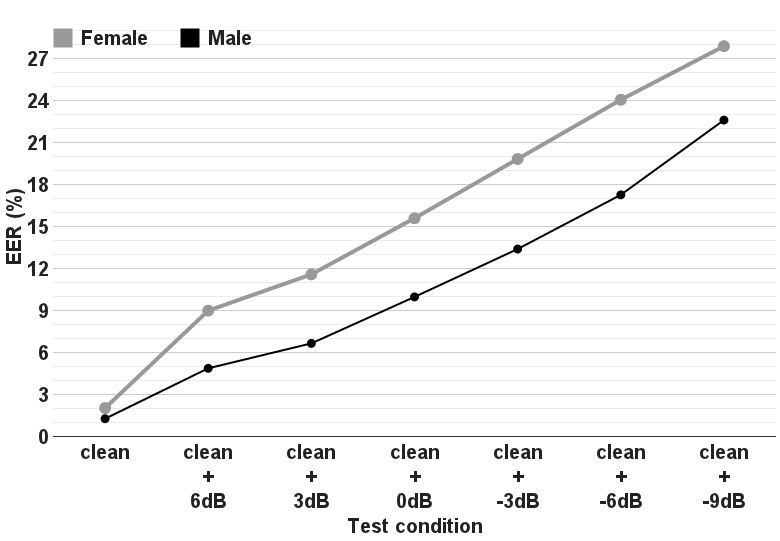
\includegraphics[height = 3.43in, width=0.9\textwidth]{figures/sidingrid_ovlintest}
	\vspace{-1mm}
	\caption{\it The rise in EER values as we increase the effect of overlapped speech (via decreasing the SIR). Starting from clean (i.e. single-speaker speech) to lower SIR values. a) Shows the case where train files are clean, but test files contain overlaps. }
	\label{fig:sidingrid_ovlintest_train_a}
\end{figure}
\begin{figure}[h!]%{0.5\textwidth}
	\centering
	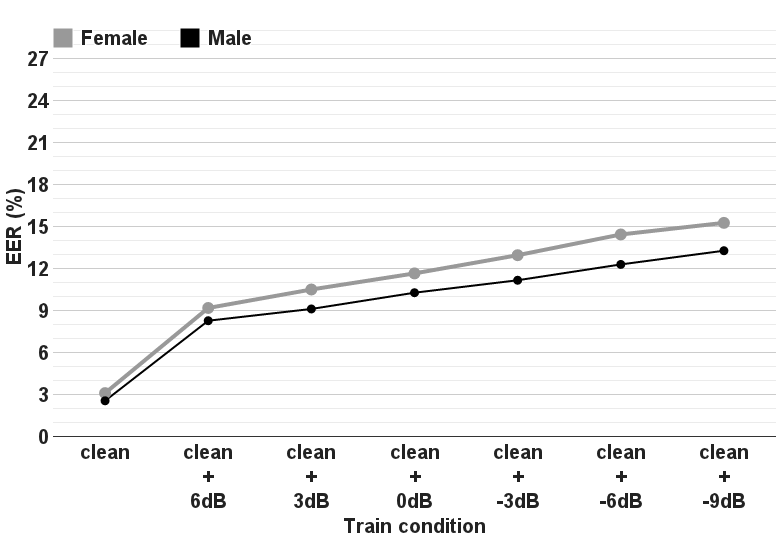
\includegraphics[height = 3.43in, width=0.9\textwidth]{figures/sidingrid_ovlintrain}
	\vspace{-1mm}
	\caption{\it b) clean test files but train files contain overlaps.}
	\label{fig:sidingrid_ovlintest_train_b}
\end{figure}



\begin{figure}[h!]
	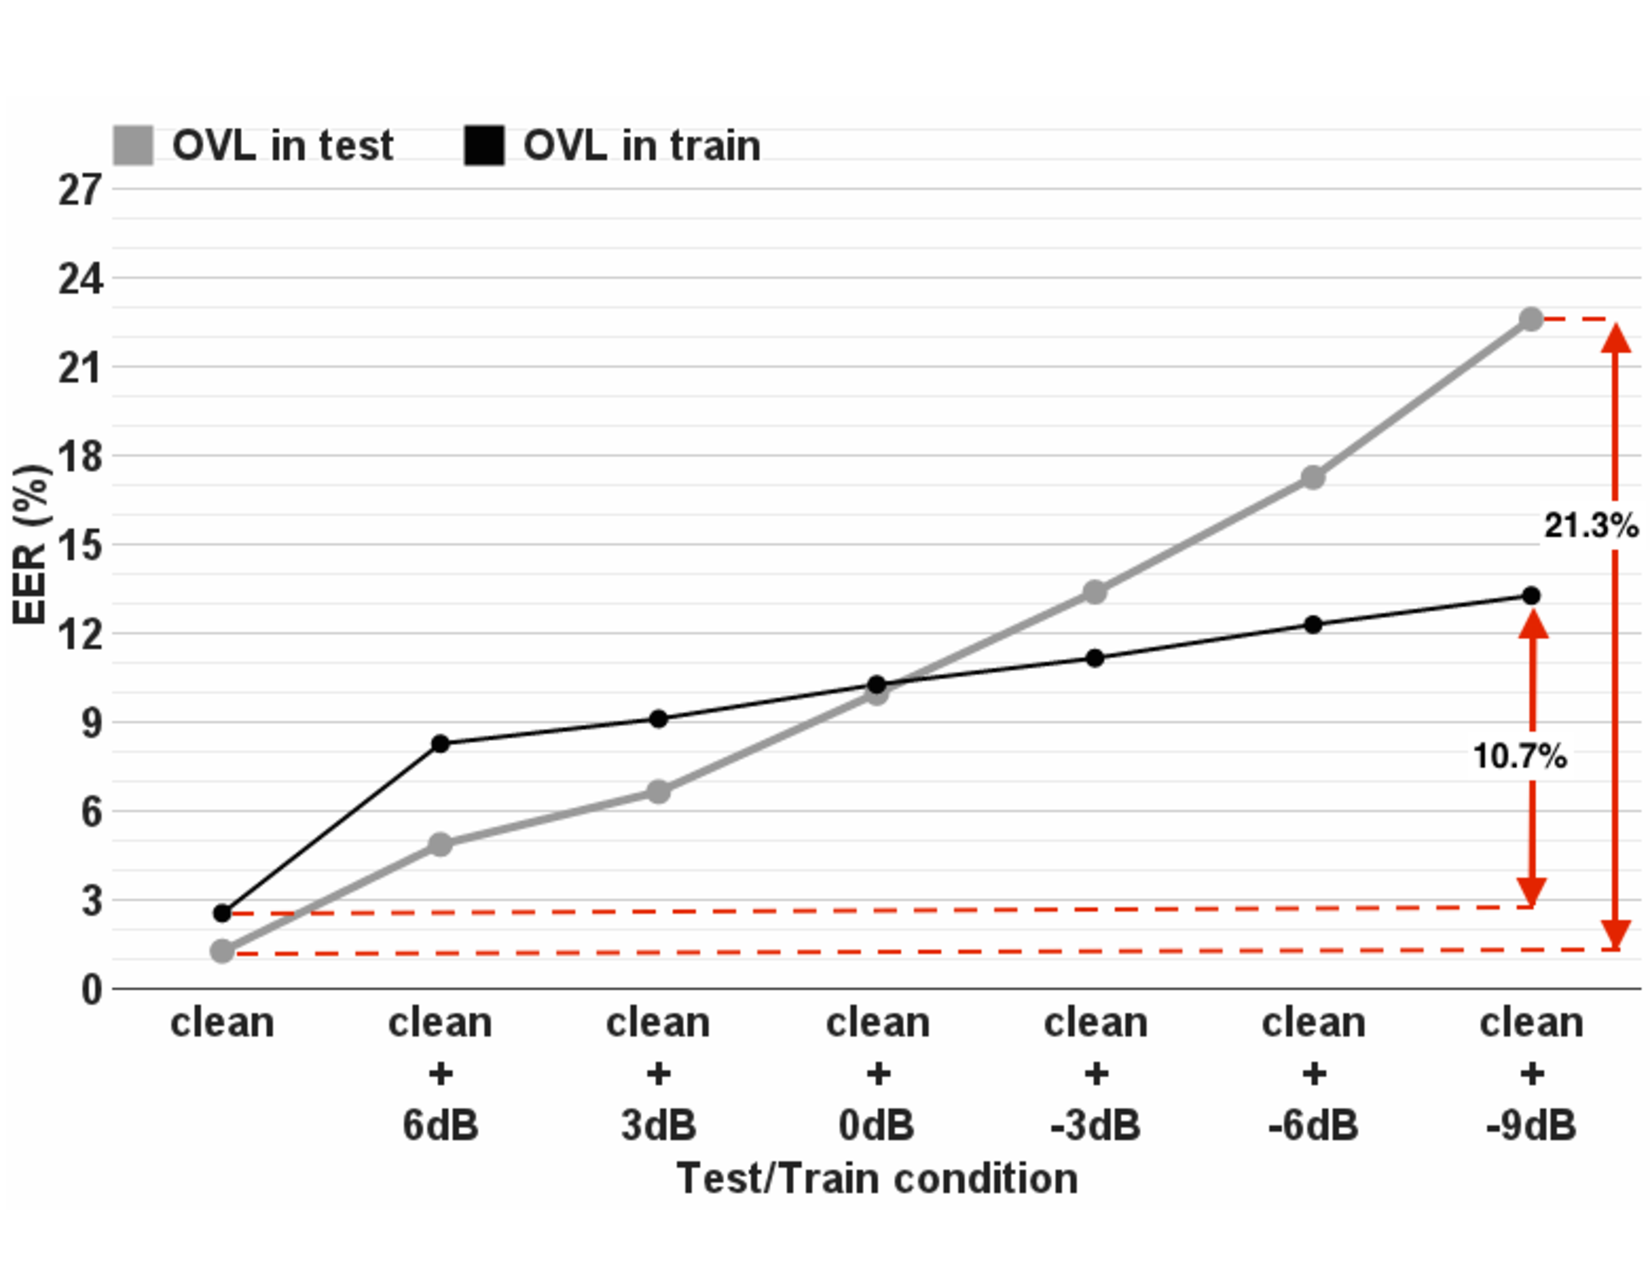
\includegraphics[height = 3.43in, width=0.9\textwidth]{figures/sidingrid_ovlintrainvstest_male_rev1}
	\caption{\it Comparing the impact of increasing overlap (OVL) in train vs. test data by decreasing SIR values. Experiments for male speakers (a). Lower SIR drops the performance more rapidly when applied to test data.}
	\label{fig:sidingrid_ovlintrainvstest_male}
\end{figure}

\begin{figure}[h!]
	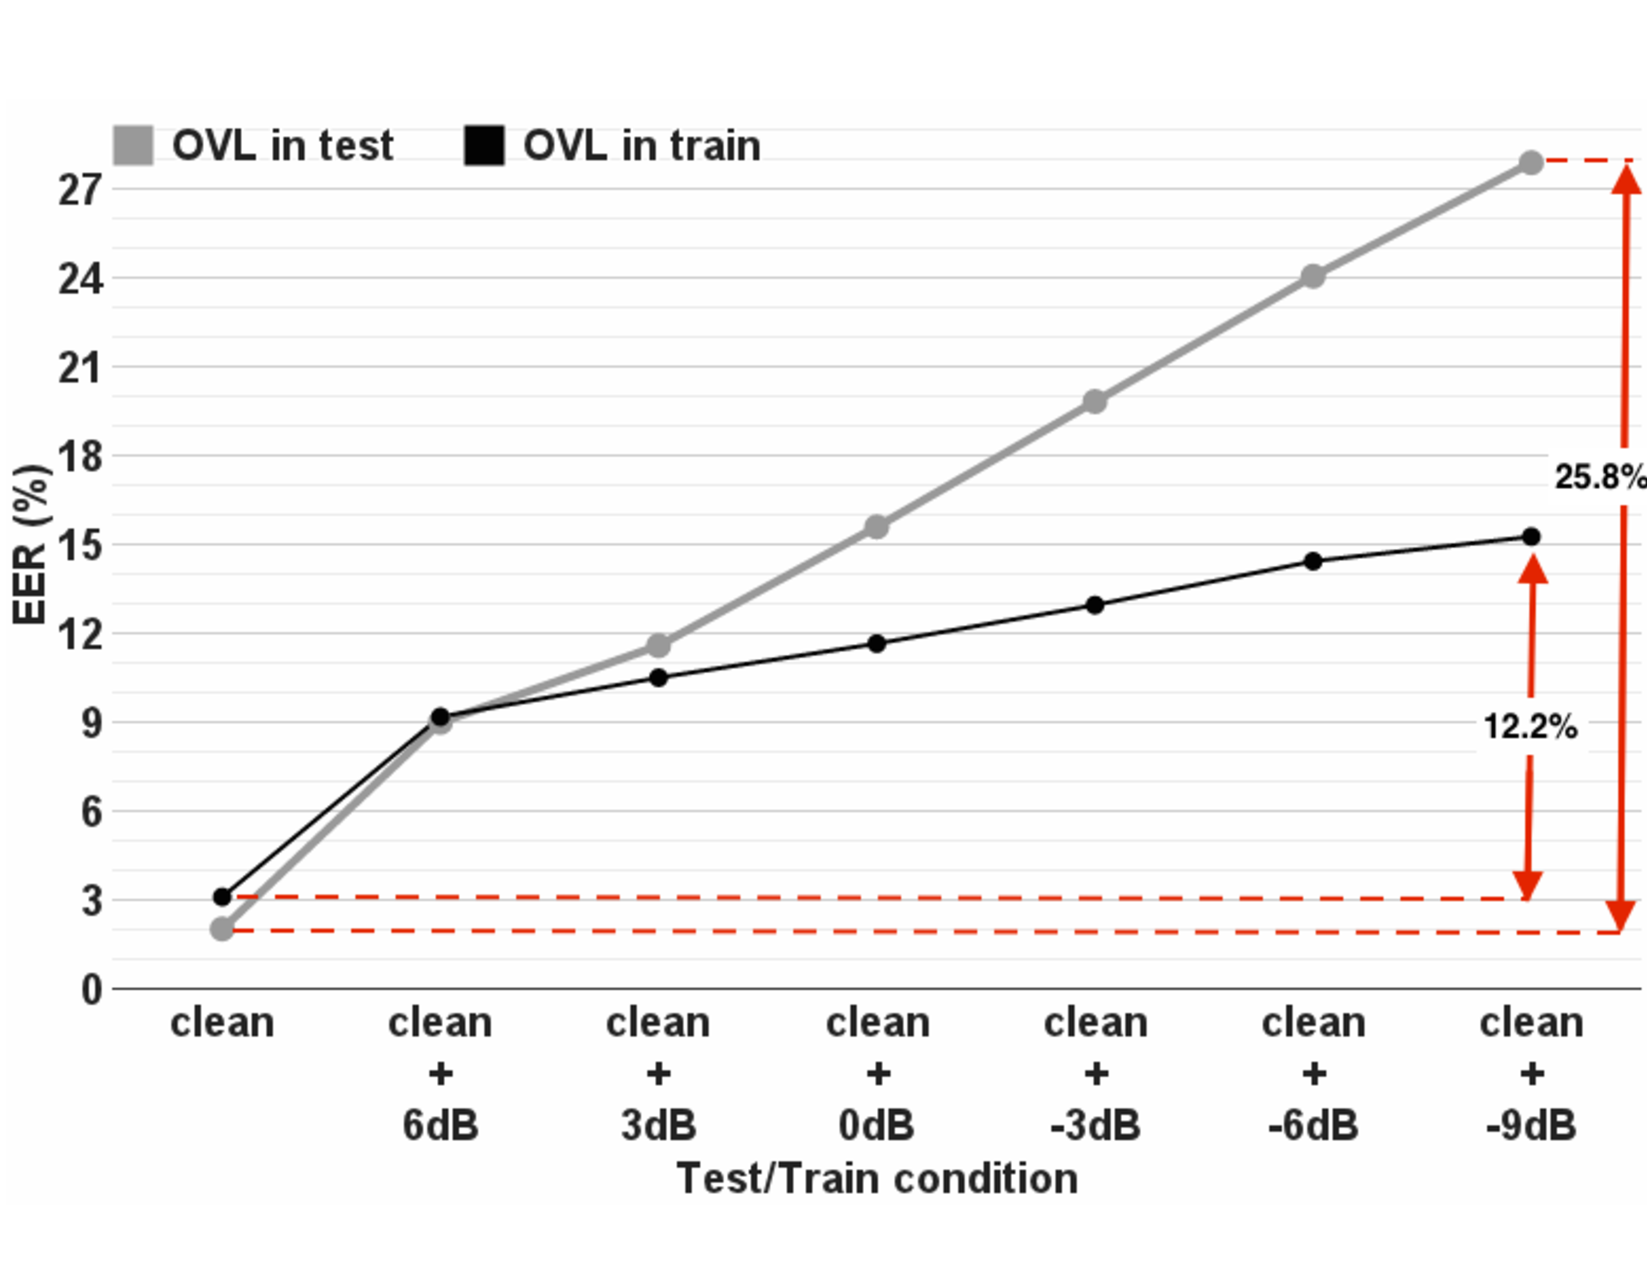
\includegraphics[height = 3.43in, width=0.9\textwidth]{figures/sidingrid_ovlintrainvstest_female_rev1}
	\caption{\it b) female}
	\label{fig:sidingrid_ovlintrainvstest_female}
\end{figure}


The results provided in Sect.~\ref{sec:ch3_OvlinTest}~and~\ref{sec:ch3_OvlinTrain} were provided to focus explicitly on the impact of overlaps on speaker verification. 
This is believed to be novel from two perspectives: 
1) The data used here is actually overlapped, meaning that files contain two speakers speaking at the same time, and not the generic case of co-channel. Therefore, the results provide greater motivation and direction as we move on to the next sections, which focus on overlap detection. 
2) The comparison made between adding overlap to test vs. training data provides insight in determining which (train or test) to prioritize for to remove overlap. Bare in mind that simply removing everything that is assumed to be overlapped does not necessarily yield optimal performance, since losing data lowers model reliability and the number of test features used to calculate likelihood values. 


\section{Overlap detection as meta-data for speaker recognition}
\label{sec:ch2_OvlQualityMeasure} 
Using meta-data to yield more accurate decisions is a common practice in speaker verification evaluations~\cite{bosaris,qual_sid_13}. 
Incorporating quality measures such as speech activity detection (SAD) and effective file durations can significantly improve verification performance~\cite{qual_sid_13,CRSSSRE12} regardless of system architecture (be it i-vector, GMM-UBM, or any other system). 
Quality measure refers to additional information (i.e. meta-data) used alongside speaker verification likelihood ratios (aka speaker verification scores) to quantify the test and train conditions in trials. 
Meta-data provides lower-level scores that help increase distinguishability between target/imposter trials. 
For speaker verification in overlapped speech, the primary source of confusion is caused by the presence of interfering speakers. 
This section proposes to use scores from overlap detection algorithm(s) as secondary information to improve overall speaker verification performance. 

There are several approaches through which quality measures can be applied in a binary classification scenario~\cite{bosaris,ietqstack,kelly2013}. 
Here, we use a stacking approach, called Q-stack, in which the quality measures (here overlap decisions) are concatenated (i.e., ``stacked'') with speaker verification decisions~\cite{ietqstack}. 
The resulting vector is a high-dimensional score vector which allows more separability due to the additional information provided by the stacked dimensions. 
The stacked score vectors are then processed with a support vector machine (SVM) classifier. 
SVM parameters are trained using a development set extracted from a separate subset of the data. 
In experiments, the development set consists of $10,000+$ trials, a quarter of which are clean trials and the remaining $7,500+$ trials contain overlapped test files with $0,3,6dB$ SIR levels. 
The target to imposter ratio in speaker verification trials is $0.001$. 
An evaluation set of size $18,000$ trials with similar specifics and target-imposter ratio is used to test overall system performance.


Table~\ref{tab:sid_stack_results} shows the improvements obtained by using the overlap detection scores individually and combined. 
Kurtosis and SFM show less correlation, however they provide significant complementary information when combined and used alongside SAPVR and pyknogram features. 
The best result is obtained when all four features are concatenated, since each overlap detection system may yield better performance in certain scenarios.  


\begin{table}[t]
	\centering
	\begin{tabular}{|c|c|c|c|c|c|}
		\hline
		raw GMM/UBM scores & pykno & kurtosis & SFM & SAPVR & $\textit{\textbf{EER (\%)}}$ \\ \hline
		\cellcolor[HTML]{C0C0C0}{\color[HTML]{343434} } \checkmark &  &  &  &  & 11.36\\ \hline \hline
		\cellcolor[HTML]{C0C0C0} \checkmark & \cellcolor[HTML]{C0C0C0} \checkmark &  &  &  & 10.19 \\ \hline
		\cellcolor[HTML]{C0C0C0} \checkmark &  & \cellcolor[HTML]{C0C0C0} \checkmark &  &  & 13.51 \\ \hline
		\cellcolor[HTML]{C0C0C0}{\color[HTML]{343434} } \checkmark &  &  & \cellcolor[HTML]{C0C0C0}{\color[HTML]{343434} } \checkmark &  & 28.35 \\ \hline
		\cellcolor[HTML]{C0C0C0} \checkmark &  &  &  & \cellcolor[HTML]{C0C0C0} \checkmark & 9.48 \\ \hline \hline
		\cellcolor[HTML]{C0C0C0}{\color[HTML]{343434} } \checkmark & \cellcolor[HTML]{C0C0C0} \checkmark & \cellcolor[HTML]{C0C0C0}{\color[HTML]{343434} } \checkmark &  &  & 10.20 \\ \hline
		\cellcolor[HTML]{C0C0C0} \checkmark & \cellcolor[HTML]{C0C0C0} \checkmark &  & \cellcolor[HTML]{C0C0C0} \checkmark &  & 10.47 \\ \hline
		\cellcolor[HTML]{C0C0C0} \checkmark & \cellcolor[HTML]{C0C0C0} \checkmark &  &  & \cellcolor[HTML]{C0C0C0} \checkmark & 9.57 \\ \hline \hline
		\cellcolor[HTML]{C0C0C0} \checkmark & \cellcolor[HTML]{C0C0C0} \checkmark & \cellcolor[HTML]{C0C0C0} \checkmark & \cellcolor[HTML]{C0C0C0} \checkmark &  & 10.31 \\ \hline
		\cellcolor[HTML]{C0C0C0} \checkmark & \cellcolor[HTML]{C0C0C0} \checkmark & \cellcolor[HTML]{C0C0C0} \checkmark & \cellcolor[HTML]{FFFFFF} & \cellcolor[HTML]{C0C0C0} \checkmark & 9.18 \\ \hline
		\cellcolor[HTML]{C0C0C0} \checkmark & \cellcolor[HTML]{C0C0C0} \checkmark & \cellcolor[HTML]{C0C0C0} \checkmark & \cellcolor[HTML]{C0C0C0} \checkmark & \cellcolor[HTML]{C0C0C0} \checkmark & {\bf 9.10}\\ \hline
	\end{tabular}
	\caption{\it Speaker verification performance (EER) with and without overlap detection scores as meta-data. Grey cells highlight the features used in each experiment. The relative change in EER is presented in the last column.}
	\label{tab:sid_stack_results}
	\vspace{-5mm}
\end{table}

\vspace{0mm}

% The following paragraph was added after reviewer1's comments (and also reviewer 3):
Better individual performances from SAPVR and SFM is because they are superior in distinguishing harmonic structures. 
Since speaker identities are mostly influenced by voiced speech, this assists the speaker recognition task in quantifying the amount of reliable voiced segments. 
Pyknogram-based detection is designed to locate harmonic discontinuities as opposed to the presence of harmonics. 

Experiments show that the best performance is obtained using an SVM with a radial basis function (RBF) kernel. 
The SVM parameter(s) (here $\gamma$) are determined through cross-validation on the development set. 
Class weights (i.e., target/imposter weights for the SVM classifier) and the cost (aka slack) parameter are selected according to the detection cost function (DCF) parameters ($C_{fa}$, $C_{miss}$, and $prior$) used throughout experiments~\cite{bosaris}. %Table~\ref{tab:sid_stack_results}  The highest relative improvement is obtained when all features are concatenated. 

An additional experiment is also conducted using ideal overlap labels (labels from ground-truth) in the Q-stack paradigm which results in an lower bound in error rates.
The EER for this lower bound is $8.74\%$ ($23\%$ relative improvement). 
In the Q-stack algorithm, the relative drop in EER from using all overlap features is approximately $20\%$, which is not far off from when ground-truth labels are used. 
This confirms the effectiveness of the selected overlap detection features/scores.  
Using the proposed Pyknogram-based overlap detection system and baseline features the relative improvement is $20\%$, a mere $3\%$ lower than the best achievable performance provided by the lower bound.


\section{Summary}
\label{sec:ch3_summary}
Chapter~\ref{chapter:ovl_in_sid} provides an investigative study of overlapped speech in speaker recognition systems. 
This effect was measured by adding overlapped speech to training and test data in a speaker recognition problem. 
Since the focus in this chapter was on physical attributes of overlapped speech, all experiments were conducted on independent cross-talk data (as defined in Chapter~\ref{chap:intro}). 
It is shown that overlapped speech is more detrimental when added to test data, due to its impact on the final verification score. 
When overlap is added to training data, the effect of interfering speech is mitigated as the different secondary speakers are averaged out across training sessions provided for a given speaker. 
A proposed method to decrease the impact of overlapped speech is to use overlap detection scores as meta-data for a speaker verification system. 
The traditional approach has been to simply remove overlapped segments. 
Alternatively, this study investigates the improvement obtained by preserving data (be it overlapped or not) while calibrating speaker verification scores to adjust to various levels of overlap in test and training data. 
